\chapter{MD Realtime Record Page:}

The RTRK Page is used to record tracks in real-time. If the sequencer is running, trigger presses on the MD will be recorded.

Thanks to micro-timing, trigger presses are recorded at 1/192th note resolution and have a much more organic feel than the MD’s real-time record mode.
\screenshot{record.png}
\\
\textit{To enter RTRK Page: First select desired track on the MD \textbf{[Function + Track N]}. Then press \textbf{[PageSelect + Trigger 6]}.}

%\fbox{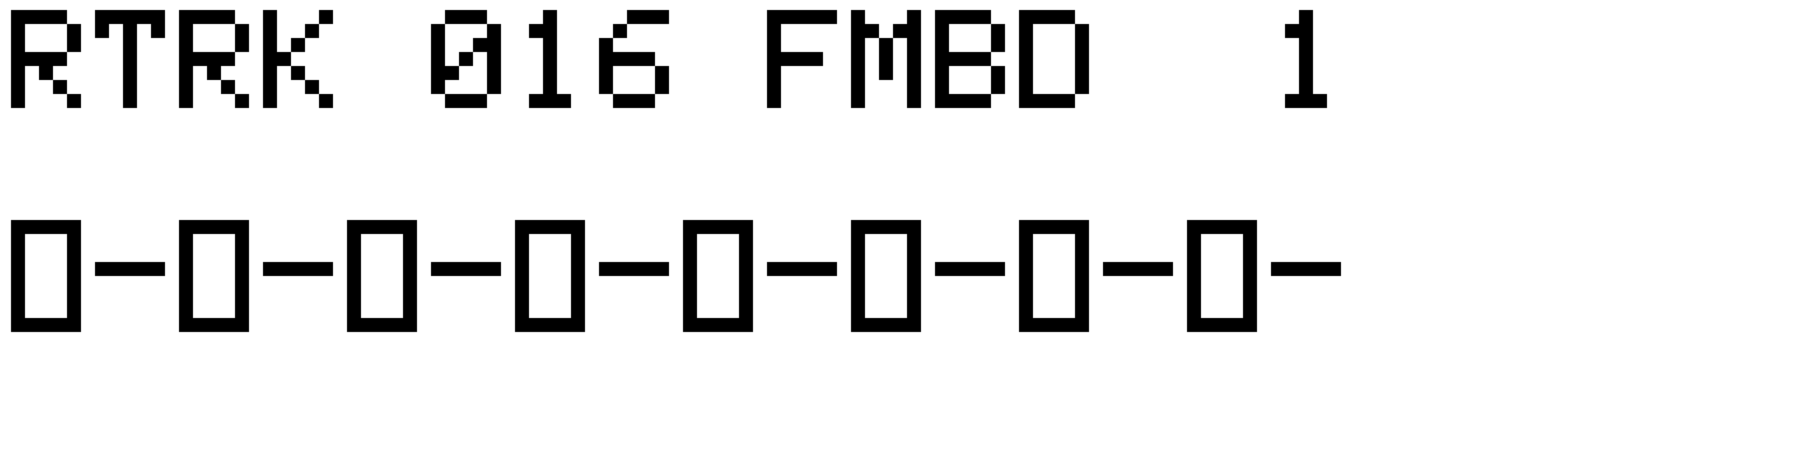
\includegraphics[scale=.40]{rtrk_page.png}}
\screenshot{rtrk_action.png}

When in RTRK Page, the current sequencer Track will automatically change according to the track corresponding to the last MD Trigger pressed.\\
\\To minimise record latency the display is prevented from updating unless a GUI action occurs. 

\encodersbuttons{--}{--}{Track Length}{--}{Toggle RTRK/RLCK}{PageSelect}{Rotate View}{Track/Trig Menu}

\section{Clearing a sequence:}
\begin{itemize}
\item To clear the current track, press and hold the\textbf{ [ Shift2 ]} to open the track menu, rotate \textbf{[Encoder2]} to the entry \textbf{CLEAR}, then rotate \textbf{[Encoder1]} to select \textbf{TRK}.
\item To clear all MD tracks, select \textbf{ALL}
\end{itemize}

\vspace{-0.3cm}

\section{Rotating visible sequence:}
Each track consists of 4 pages of 16 steps, for a total of 64 steps per track.
\begin{itemize}
\item Rotate the current track-page by pressing the \textbf{[Write] }button.
\end{itemize}

\vspace{-0.3cm}

\section{Changing track length:}
\begin{itemize}
\item Track length is controlled by rotating \textbf{[ Encoder 3 ]}. Only steps less than the current track length are drawn.
\item To change the lengths of all 16 tracks simultaneously hold down \textbf{[Write]} whilst rotating \textbf{[ Encoder 3 ]}.
\item Track length can also be set by holding \textbf{[Write]} and then selecting the corresponding step from the MD trigger interface. The track length is offset by the current track-page.
\end{itemize}

